\chapter{Application}\label{app}
This chapter will describe how browser extensions are built in google chrome, focusing on architecture and security features. Browser extensions can be utilized to build an application implementing "human computable passwords" as described in \autoref{ch:hcp}. The scheme is different from other traditional password managers since it does not \emph{store} the password, but challenges \emph{helping} the user to remember strong passwords. The idea by using browser extensions to implement this is to have an extension monitor the password fields of the sites a user visits and update the challenges depending on the current state of the active site. This technique will be described and a prototype extension demonstrated. 
\section{Browser Extensions}\label{browser-extensions}
Modern computer users shift towards doing more and more work through their web browsers. Web applications have become popular due to the ubiquity of browsers, thus allowing web apps to run anywhere. A web app can run at any platform running a web browser, allowing the application to run on multiple platforms as well as different devices. Updates can be applied quickly without having to distribute patches to a possibly huge amount of devices.
\par Browser extensions add additional features to the web browser allowing the user to tweak the experience of the web pages visited. Typical examples are extensions adding to, or tweaking already present features of the browser such as changing how bookmarks are managed, or adding additional features such as blocking advertisements. Lately browser extensions have been extended even further allowing standalone applications to be developed running as native applications \footnote{A new breed of Chrome apps, \url{http://chrome.blogspot.no/2013/09/a-new-breed-of-chrome-apps.html} - accessed: 2015-03-02}. This allows developers to create desktop apps using the same technology as in web apps, mainly HMTL5, Javascript and CCS.
\par This chapter will present Google chrome browser extensions, including architecture and security mechanisms.

%This project will utilize chrome extensions to create a password manager running in the browser. 
%The user interface will be in a panel spawned by a browser action activated when the user click the icon in the navbar. 
%The user interface is built using the open-source web application framework AngularJS \cite{angularjs}, storage is done using the chrome local storage API.

\subsection{Extension Security}\label{extension-sec}
\par Browser extensions introduce some security concerns which must not be forgotten while developing applications using this environment. Chrome extensions run in the browser with access to both the \gls{dom} of the active page as well as the native file system and connected devices. The overall architecture of the application is summarized in \autoref{extension-architecture} and described in the chrome extensions documentation \footnote{What are extensions?, \url{https://developer.chrome.com/extensions/overview} - accessed 2015-03-02}. This section will describe the architecture considering security concerns relevant when developing chrome extensions which handle sensitive data such as passwords.

%The extension core consist of the actual application interface visible to the user as well as long running background jobs and business logic. The background page can be used to spawn panels or popups, and has access to browser APIs.  The extensions is activated through a icon in the browser navbar as seen in \autoref{extension-ux}. Clicking the icon typically spawns a popup or a panel to interact with the user. In addition to the core, each extensions can have content scripts which has access to the content of the current active web page, and can monitor and alter \gls{dom} of this. 


\begin{figure}[h]
   \fbox{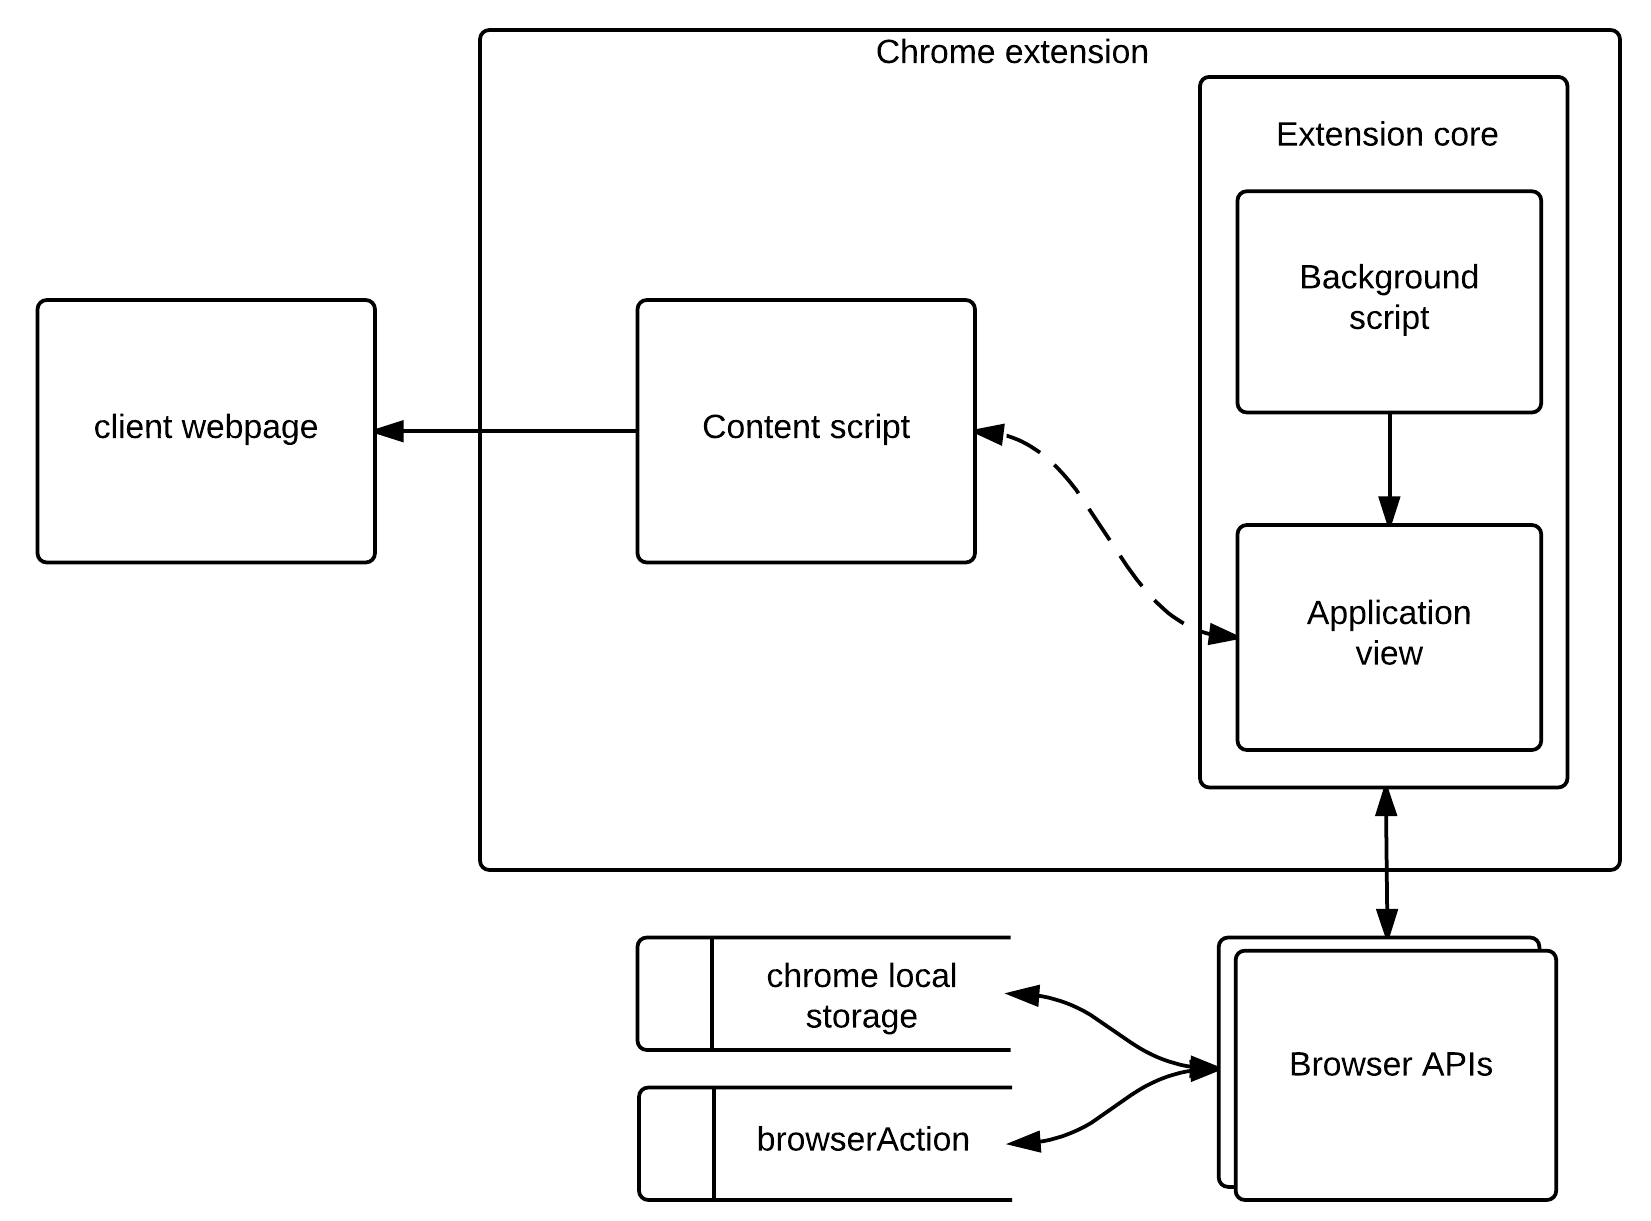
\includegraphics[width=\textwidth]{chrome-extension-architecture} }
    \caption{Chrome extension architecture.}
    \label{extension-architecture}
\end{figure}

\par Earlier extensions written for IE and Firefox ran in the same process as the browser and shared the same privileges. This made extensions an attractive entry point for attackers, since a buggy extension could leave security holes leaking sensitive information or even provide an entry point to the underlying operating system. For these browsers several frameworks for security have been proposed \cite{firefox-ie, js-info-flow}, trying to mitigate vulnerabilities is browser extensions. The chrome extensions architecture is built from scratch with security in mind. Chrome uses a permission system following three principles \cite{liu-chrome}; \emph{least privileges}, \emph{privilege separation} and \emph{process isolation}. 

\paragraph{Least privilege} specifies that extensions should only have to privileges they need functions, not share those of the browser. The privileges of each extension are requested in the \emph{manifest} file \footnote{Manifest file format, \url{https://developer.chrome.com/apps/manifest} - accessed 2015-03-04}. This json file needs to be included in all chrome extensions, and consist of all the permissions needed by the extension as well as some meta data and version information. This is done to prevent compromised extensions from exploiting other permissions than those available at runtime. An example of a manifest file can look like this: 

\begin{verbatim}
{
    "name": "Example extensions",
    "description": "An example extensions to demonstrate how the
                    manifest file works.",
    "version": "1.2",
    "manifest_version": "2"
    "background_page": "main.hmtl",
    "permissions": [
        "bookmarks",
        "storage",
        "https://*.ntnu.no"
    ]
}
\end{verbatim}
This extension has specified access to the bookmarks API, chrome local storage and all sub domains of ntnu.no. Extensions can request different permissions in the manifest file including web site access, API access and native messaging. If an extension contains weaknesses it will not compromise any other parts of the system not covered by the specified privileges. For the least privileges approach to work properly each developer should only request the permissions needed, Barth et al. \cite{protecting-browsers} examined this behavior and concluded that developers of chrome extensions usually limit the origins requested to the ones needed. 

\paragraph{Privilege separation.} Chrome extensions are, as mentioned, divided into components; content scripts, extension core and native binaries. The addition of native binaries allows extensions to run arbitrary code on the host computer, thus posing a serious security threat. This project does not use this permission, this component will thus not be mentioned from now on. 
\par \emph{Content scripts} are javascript files allowing extensions to communicate with untrusted web content of the active web page. These scripts are instantiated for each visited web page and has direct access to the \gls{dom} of these, allowing both monitoring and editing of DOM elements. To be able to inject content scripts to a visited page, the origin of the site has to be added to the manifest file. Other than this permission, content script are only allowed to communicate with the extension core. It is important that the privileges of these scripts are at the minimum level since they are at high risk of being attacked by malicious web sites \cite{chrome-extension-dangers}, due to the direct interaction with the \gls{dom}. 
\par The \emph{extension core} is the application interface responsible for interaction with the user as well as long running background jobs and business logic. The core is written in HTML and javascript and is responsible for spawning popups and panels, as well as listening for browser action. The typical way to activate a extensions is by clicking an icon in the navigation bar, which then activates either a popup or a detached panel. The core is the components with the most privileges as it does not interact with any insecure content directly, only through direct messaging to a content script or using http requests if the target origin is defined in the manifest. 
\par In addition to this the core has access to the extension APIs, these are special-purpose interfaces providing additional features such as alarms, bookmarks, cookie and file storage. The APIs are made available through the manifest file and only those specified there can be used. \autoref{extension-ux} illustrates the interaction between the background page, content scripts, panels and active web page. The information flow starts by clicking the extension's icon in the navigation bar which launches the background page spawning a panel in the browser. A content script is injected in the current web site (google.no in the example), the script now have access to the DOM of this site and can communicate with the background which in turn can update the panel. 


\begin{figure}[h]
    \fbox{ 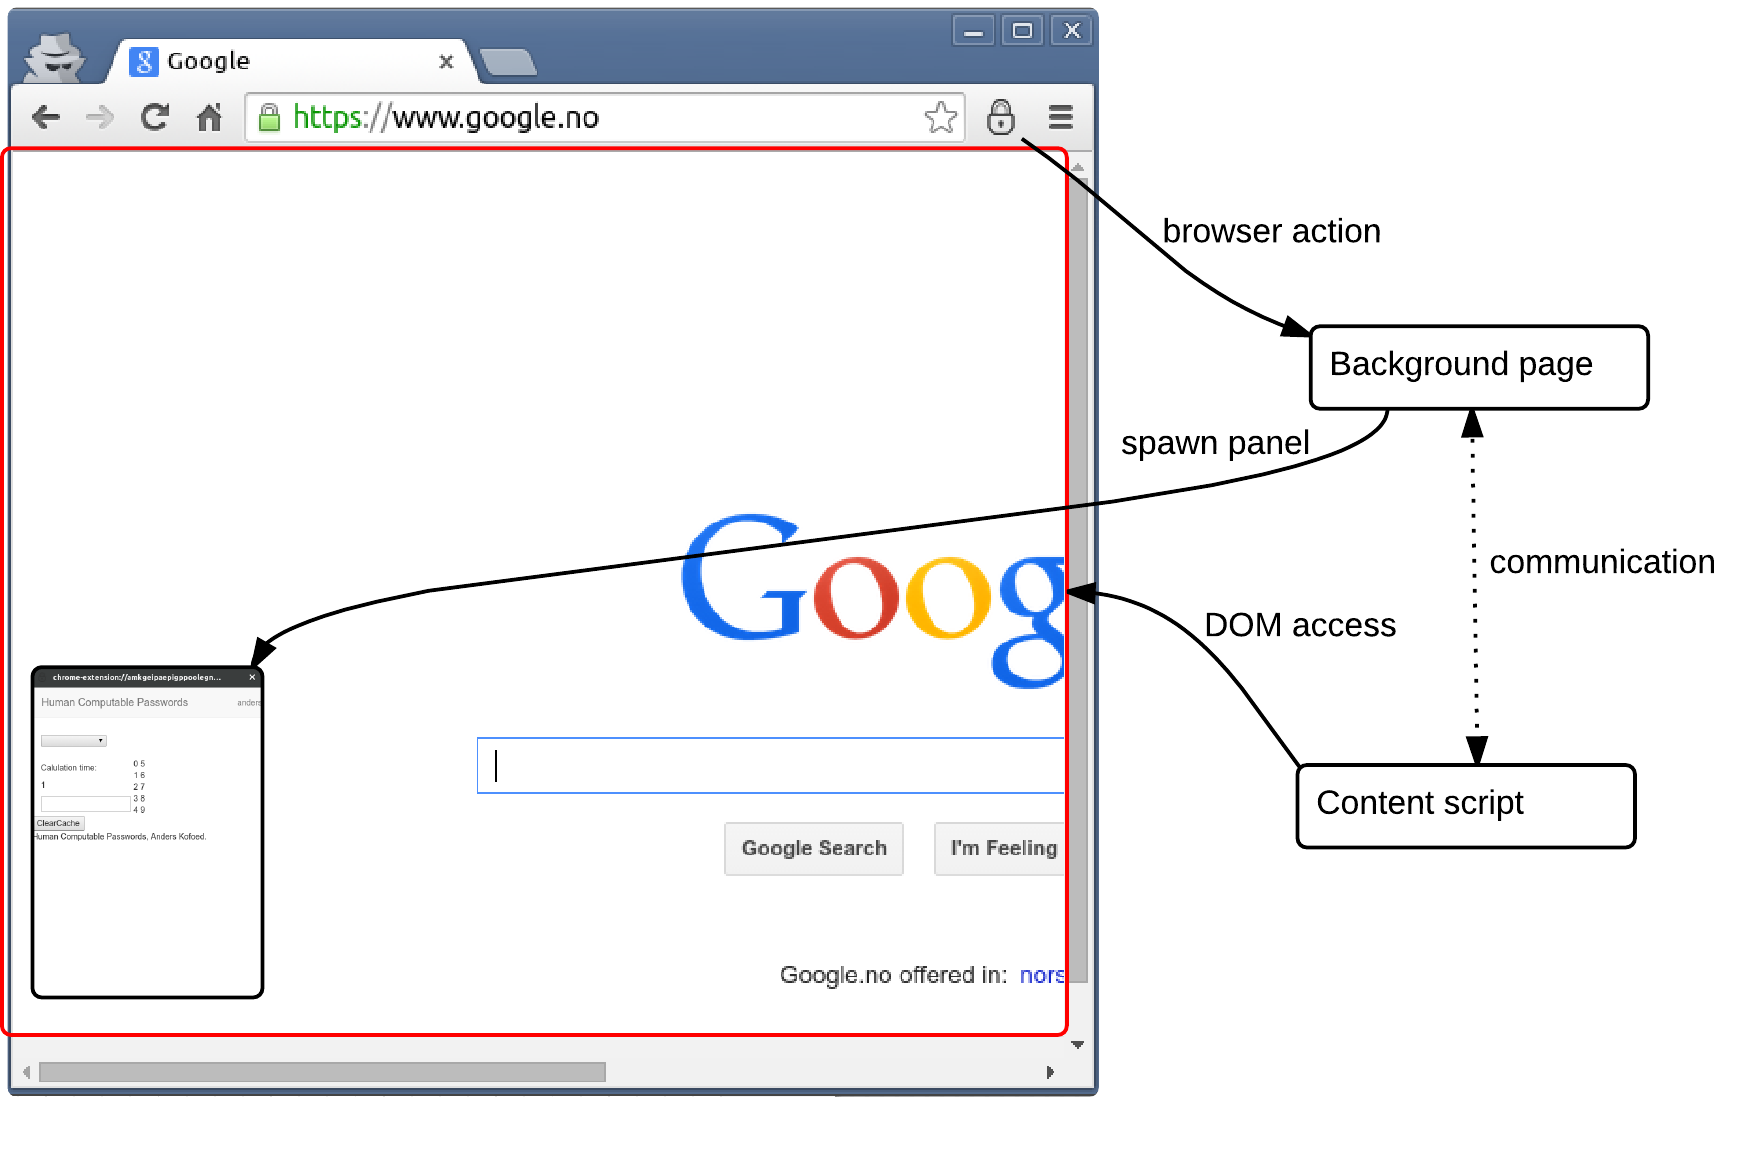
\includegraphics[width=\textwidth]{chrome-extension-ux} }
    \caption{Chrome extensions browser action and content scripts.}
    \label{extension-ux}
\end{figure}

\paragraph{Process isolation} is a set of mechanisms shielding the component from each other and from the web. Usually when javascript is loaded from the web the authority of the script is limited to the origin from where the script is loaded \cite{protecting-browsers}. Since the scripts used by the extensions are loaded from the file system, they do not have a origin in the same sense, and thus need to be assigned one. This is done by including a public key in the url of the extension, allowing a packaged extension to sign itself, freeing it from any naming authority or similar. The public key also enables usage of persistent data storage, since the origin of the extension can stay the same throughout updates and patches. This wouldn't be possible otherwise since the chrome local storage API relies on origin. \todo{more details}
\par The different components also run in different processes. The content scripts are injected and ran in the same process as the active web page, while the core run in its own process started when the extension is initiated. \todo{paragraph not finished. Cross-origin js and malicious web site operators.}
\par Finally content scripts are ran in a separate javascript environment isolating it from the possibly insecure environment of the web site. The environment of the content scripts are called isolated world, which in practice is a separate set of javascript objects reflecting the ones of the underlying DOM of the web page. This means that the content script can read and edit the DOM of the page it is injected into, but not access variables or javascript functions present in the web page. Both the page and the content scripts sees no other javascript executing in their own isolated world, but they share the same DOM \footnote{Content Scripts, \url{https://developer.chrome.com/extensions/content_scripts} - accessed: 2015-03-05}.


\section{Human Computable Passwords Chrome Extension}
\todo[inline]{Present the idea of why and how a chrome extensions can be built to realize the scheme}
Chrome extensions are very useful in that they can be ran from any computer with Google chrome installed, thus on any operating system and on any computer. An extension makes it possible to run applications while browsing the web, which in the case of an password management scheme is very useful. An application meant to help the user recall complex passwords should preferably be visible simultaneously with the password field. The most popular password management software today are usually either web applications, mobile applications or native desktop applications\footnote{Five Best Password Managers. \url{ http://lifehacker.com/5529133/five-best-password-managers }}, some of these might include plug-ins such as browser extensions. All of these password managers are reliably storing all the passwords as described in \autoref{subsec:pms}, then they are either auto-filled into the login fields or through copy pasting manually. 
\par This section will present the design and prototype implementation of the human computable password scheme (\autoref{ch:hcp}, \cite{hcp-blocki}. The design evolves around the fact that the scheme does not have to store anything securely, it is though important to make it as easy as possible for the user. The architecture will be similar to the one explained in \autoref{browser-extensions} using content scripts to monitor the password fields of the active browser session. The user interface will be presented through a "panel" in the browser. Panels are windows that stays in focus will interacting with other windows or applications \footnote{"Panels"- The Chromium Project. \url{https://www.chromium.org/developers/design-documents/extensions/proposed-changes/apis-under-development/panels}}. 




\subsection{Applications Design}
\todo[inline]{Relate the ideas and architecture presented in the previous section. Explaining how content script and local APIs will be use used to provide an extension supporting the scheme }
\todo[inline]{Models of how the extensions will look including both user interface and architecture}
The extension implementing human computable passwords \ref{ch:hcp} will be an extensions helping the user with storing and managing of challenges for different accounts. The generation of secret mappings will not be part of the application, this should be done through a separate program on the user's local computer. Such a program would follow \autoref{gen-mapping}. The requirements for the extension are the following:

\begin{itemize}
    \item Provide an user interface making it easy for the user to display challenges for different accounts.
    \item The application should keep track the active site, displaying challenges for the correct site without user interaction.
    \item Add new sites to the system easily. 
    \item Displayed challenge should update while typing the password.
    \item The user should be able to type his password directly in the password field of the active site.
    \item If the user is about to forget a secret mapping, according to the usability model \ref{sec:usability-model}, the application should notify about it and advice the user to rehearse.
\end{itemize}


\subsubsection{AngularJs}
The front-end is built and updating using AngularJS\footnote{AngularJS, \url{https://angularjs.org/}}, which is a open source, client-side javascript framework. Angular is built using a variation of the model-view-controller architecture \cite{mvc}, though the creators of angular states that angular is a model-view-whatever framework\footnote{Model-View-Whatever - \url{ https://plus.google.com/+AngularJS/posts/aZNVhj355G2 }}, point being that what the architecture is called isn't important. The \emph{view}s in angular is templates written entirely in HTML making it easy read and update. The \emph{controller} contains all the business logic used by the view. The views and controllers are connected using a shared object called \emph{\$scope}, variables or functions on this object is usually defined in the controller and accessed by the view by using double curly brackets in the view (e.g. \{\{name\}\} to access the name variable on \$scope). Figure \ref{angular-data-binding} shows how scope is used to share variables between the controller and the view. 
\par Services in angular are reusable business logic which can be used independent of the views and controllers\footnote{Services - \url{https://docs.angularjs.org/guide/services}}. Services will be used to handle variables which are shared between the view and the content scripts (explained later).

See "Angular Essentials - Rodrigo Branas"\cite{angularjs-book} for a step-by-step introduction to AngularJS.

\begin{figure}[h]
    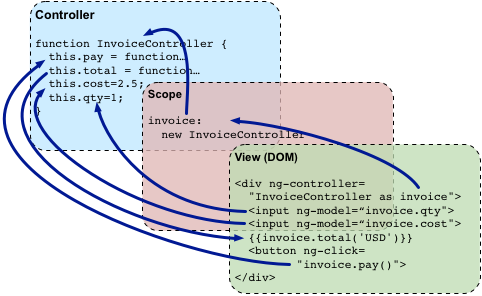
\includegraphics[width=\textwidth]{angular-data-binding} 
    \caption{Angular data binding with controller, view and scope. Figure from angular developer guide.}
    \label{angular-data-binding}
\end{figure}


\par The main benefits of using angular in this project is the data-binding which makes it easy to update the HTML shown to the user. The extension will take advantage of this when updating the challenges seamlessly while the user calculates his password.

\subsubsection{Chrome Storage.}
\emph{Local storage\footnote{Local storage - \url{ http://diveintohtml5.info/storage.html }}} is a way for applications to store data persistently and securely in the browser of clients. It is meant as an improvement of cookies which is the usual way of storing user data across sessions. The biggest problem with cookies is that they are sent with every HTTP request and thus slow down the applications using them. Local storage allows applications to store (key, value)-pairs in the browser. 
\par \emph{Chrome storage} is close to the same as local storage, differences being that chrome local storage allows applications to store data in what is called "chrome.storage.sync". This specific storage saves data locally, but also syncs it with the currently active chrome account, thus allowing a user to log into his account in any chrome browser and access the same application data. Chrome storage also allows storage of objects compared to local storage which only allows storing strings. This project will use chrome storage to persistently store challenges across sessions, and also provide backup. This way each user will be able to keep challenges for all their account within the storage of their google account. This is a important feature since it allows access to the challenges from remote locations as well.

\subsubsection{Content Scripts.}\label{cs}
Content scripts are javascript files running in the context of the active web page, as browsed by the user. These scripts has direct access to the content of the active site and can thus monitor and attach event listeners.The content scripts are isolated from the extension itself as describe in \autoref{extension-sec}, thus protecting the extension from possibly harmful sites trying to exploit weaknesses in the content script. Because of this the content scripts has to communicate with the extension through google chrome's built-in message passing system. Chrome message passing\footnote{Chrome message passing - \url{https://developer.chrome.com/extensions/messaging}} allows script to listen for and respond to messages. One side set up an event listener listening for messages, when a message is sent from the other side this event triggers and the message can be received and parsed. 
\par The content scripts and the message passing system are the only likely points of attack for adversaries. The content script can monitor the value of the password field and thus, in theory, steal these if a malicious script was able to trick it into leaking these. The communication channel is not particularly prone to attacks since even if an adversary eavesdropped all data sent on it, the only information leaked would be the current length of the password. It is though important that the design is like this since the mistake of sending the whole password string, which might seem like a solution, would be potentially dangerous. 
\par Typical usage of content scripts in this application will be to attach event listeners to the password fields of the pages visited by the user, and message the extension when the value of the password field changes. When a change happens, the content script send a message containing the current length of the typed password, so that the extension can display the correct challenge. In example if the user has entered 4 characters of his password the extension should display the 5th challenge etc. The content script also keep the extension updated on the URL of the current page, by sending a message every time a page is loaded. The extension then displays the challenges corresponding to the password of that site. If the site does not have challenges stored by the application, the user can generate new ones and store these in the system through clicking a button.  
\par See \autoref{app:content-script} for the content script file with a brief description of the code in it.

\subsection{User interface}
The user interface will be very simple, there will be two possible screens displayed to the uses. Either challenges associated to the current page will be shown, or a dialog asking the user to generate new challenges. The most important feature of the user interface is that it will automatically update depending on what site the user is currently browsing, and display the correct challenge when typing passwords. Wireframes illustrating the page schematics of the extension are shown in figures \ref{add-new-screen} and \ref{challenge-screen}.

\begin{figure}[h]
    \centering
    \begin{subfigure}[t]{0.49\textwidth}
        \centering
        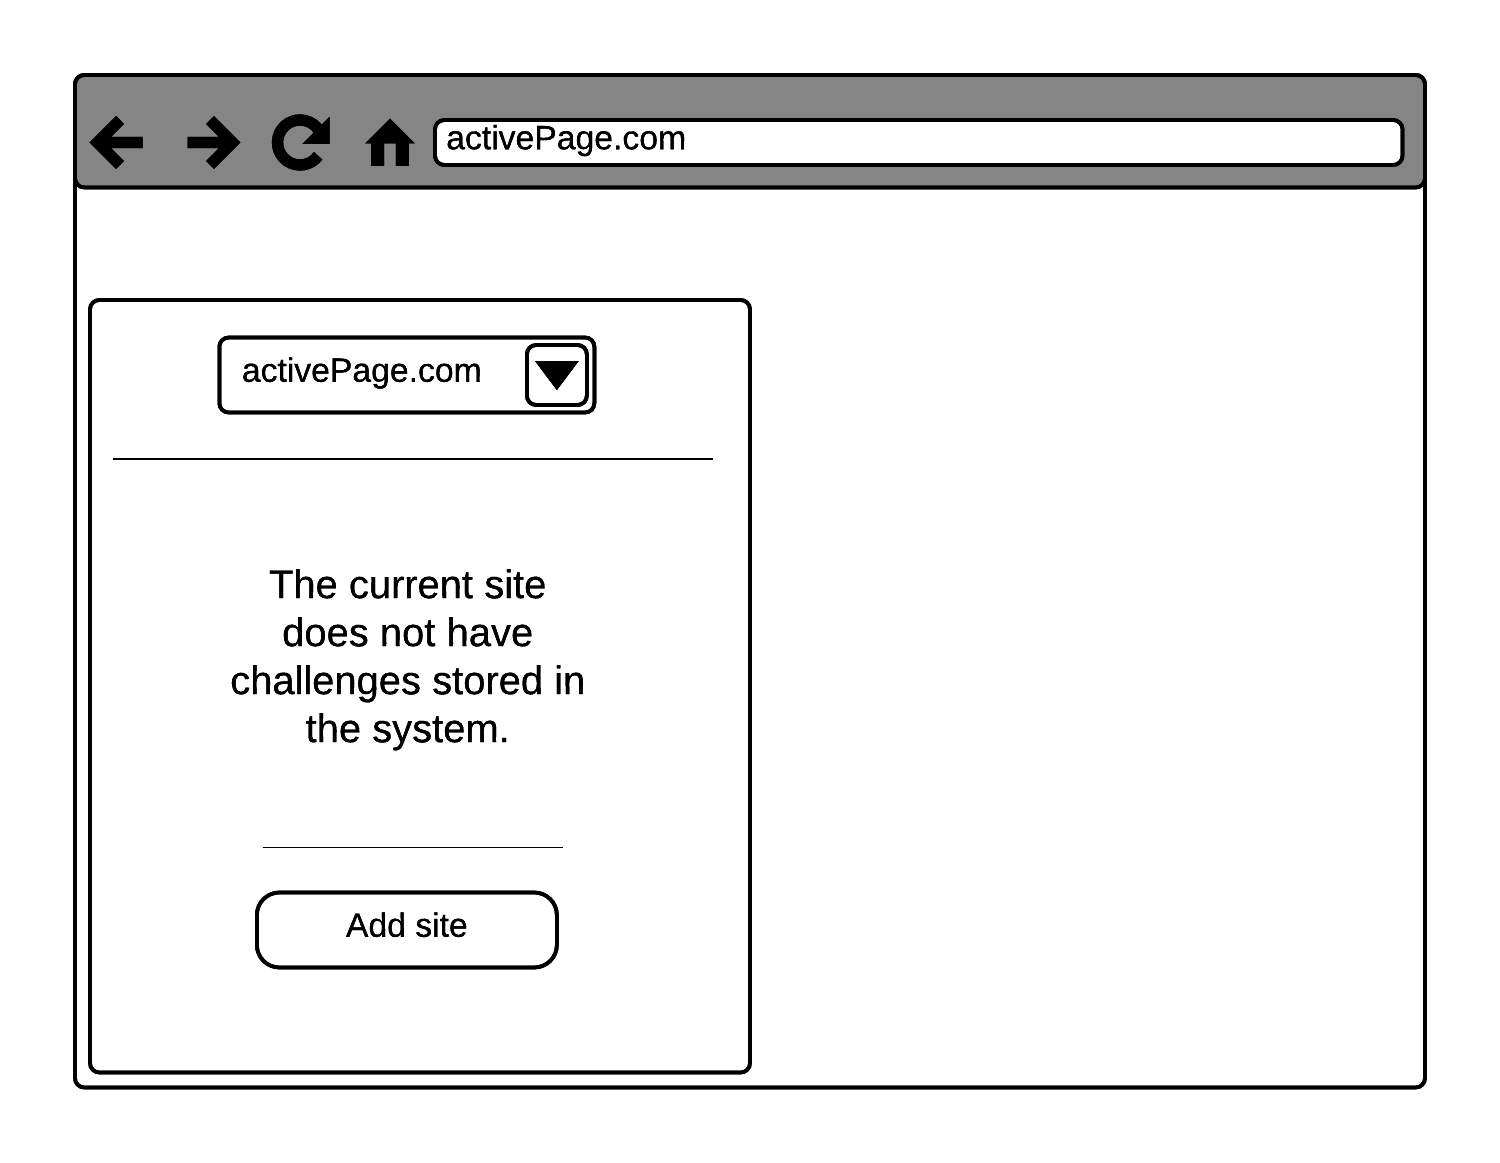
\includegraphics[width=\textwidth]{wireframe} 
        \caption{Screen seen by the user when launching the extension when visiting a page that is not stored in the system.}
        \label{add-new-screen}
    \end{subfigure}
    \hfill
    \begin{subfigure}[t]{0.49\textwidth}
        \centering
        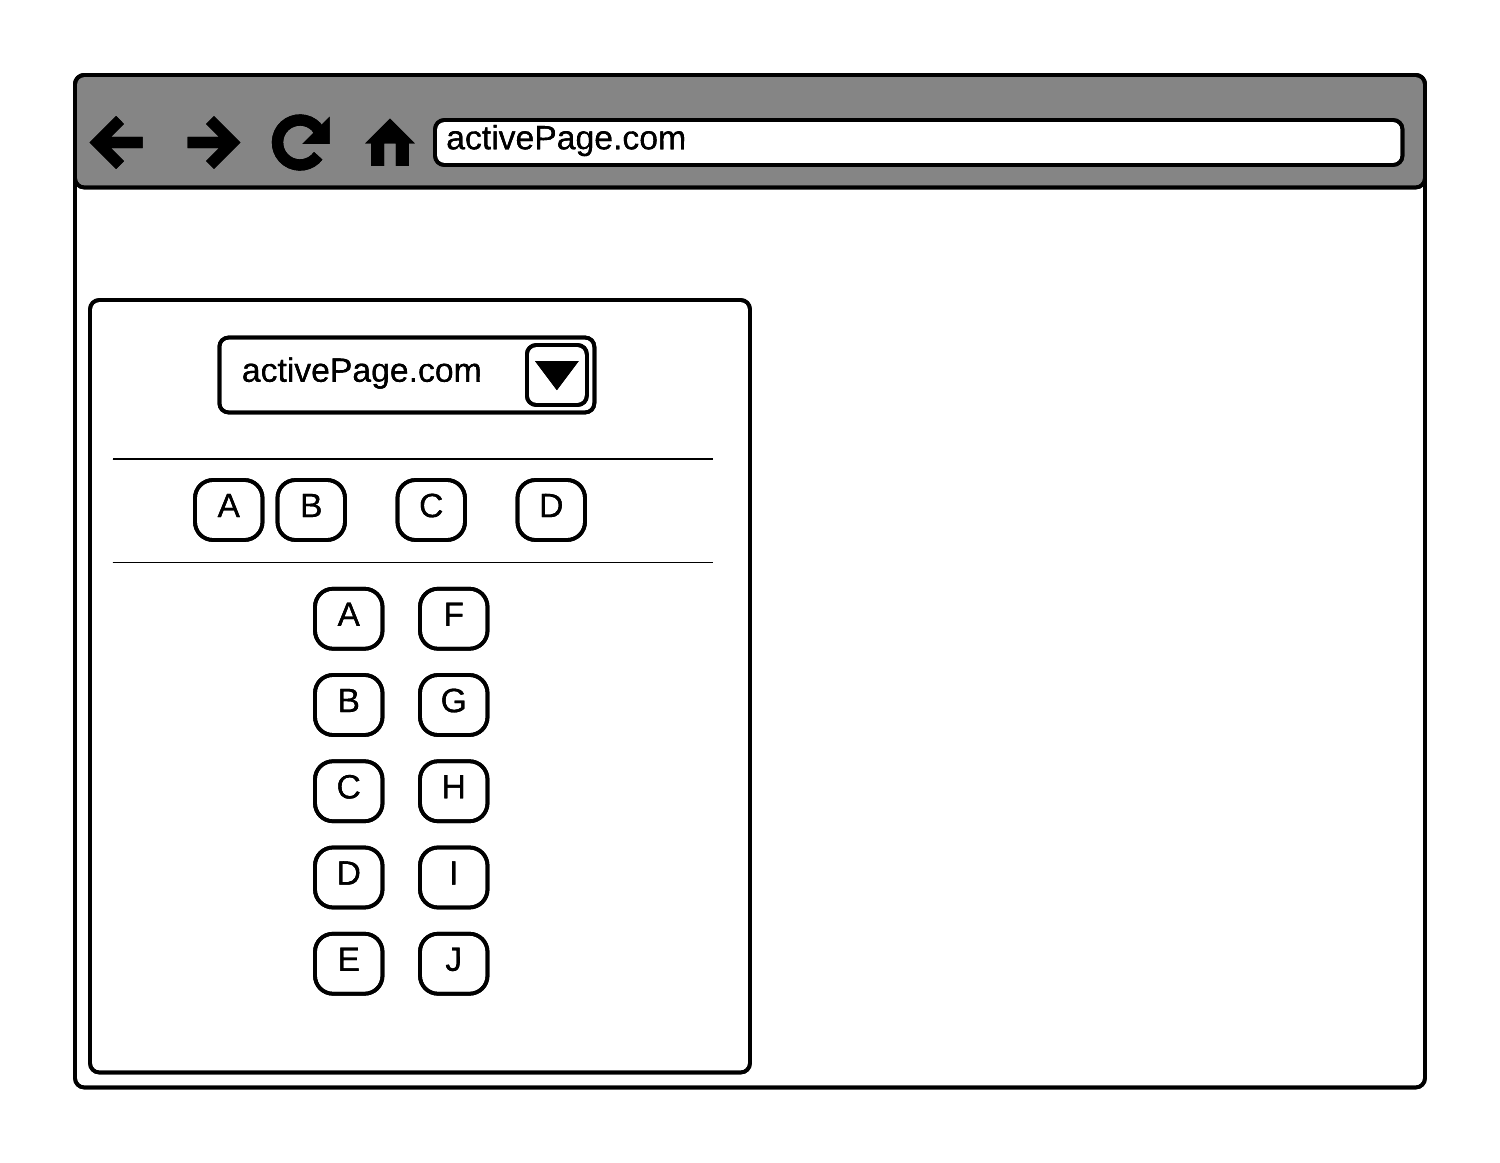
\includegraphics[width=\textwidth]{wireframe2} 
        \caption{Screen seen by the user when loading a site with challenges stored in the system. }
        \label{challenge-screen}
    \end{subfigure}
    \caption{Wireframes illustrating the page schematics of the extension.}
    \label{wireframes}
\end{figure}

\subsection{Implementation}
\todo[inline]{Present the actual design and choices made}
\todo[inline]{Demonstration of how the extension works in practice.}
\todo[inline]{Walkthrough of setting up/authenticating with an account using the scheme and the extension. }

\subsection{Architecture}
\par \autoref{class-diagram} shows the complete architecture of the system.
 The content script attach an event listener to the password field of the active site. If the content of the password field changes, the script sends a message using chrome message passing containing the current length of the password. The controller receives the new password length through the data service, and update the challenges displayed to the user. The data service is also responsible for updating the URL field accessible to the controller.

\begin{figure}[h]
    \centering
    \fbox{ 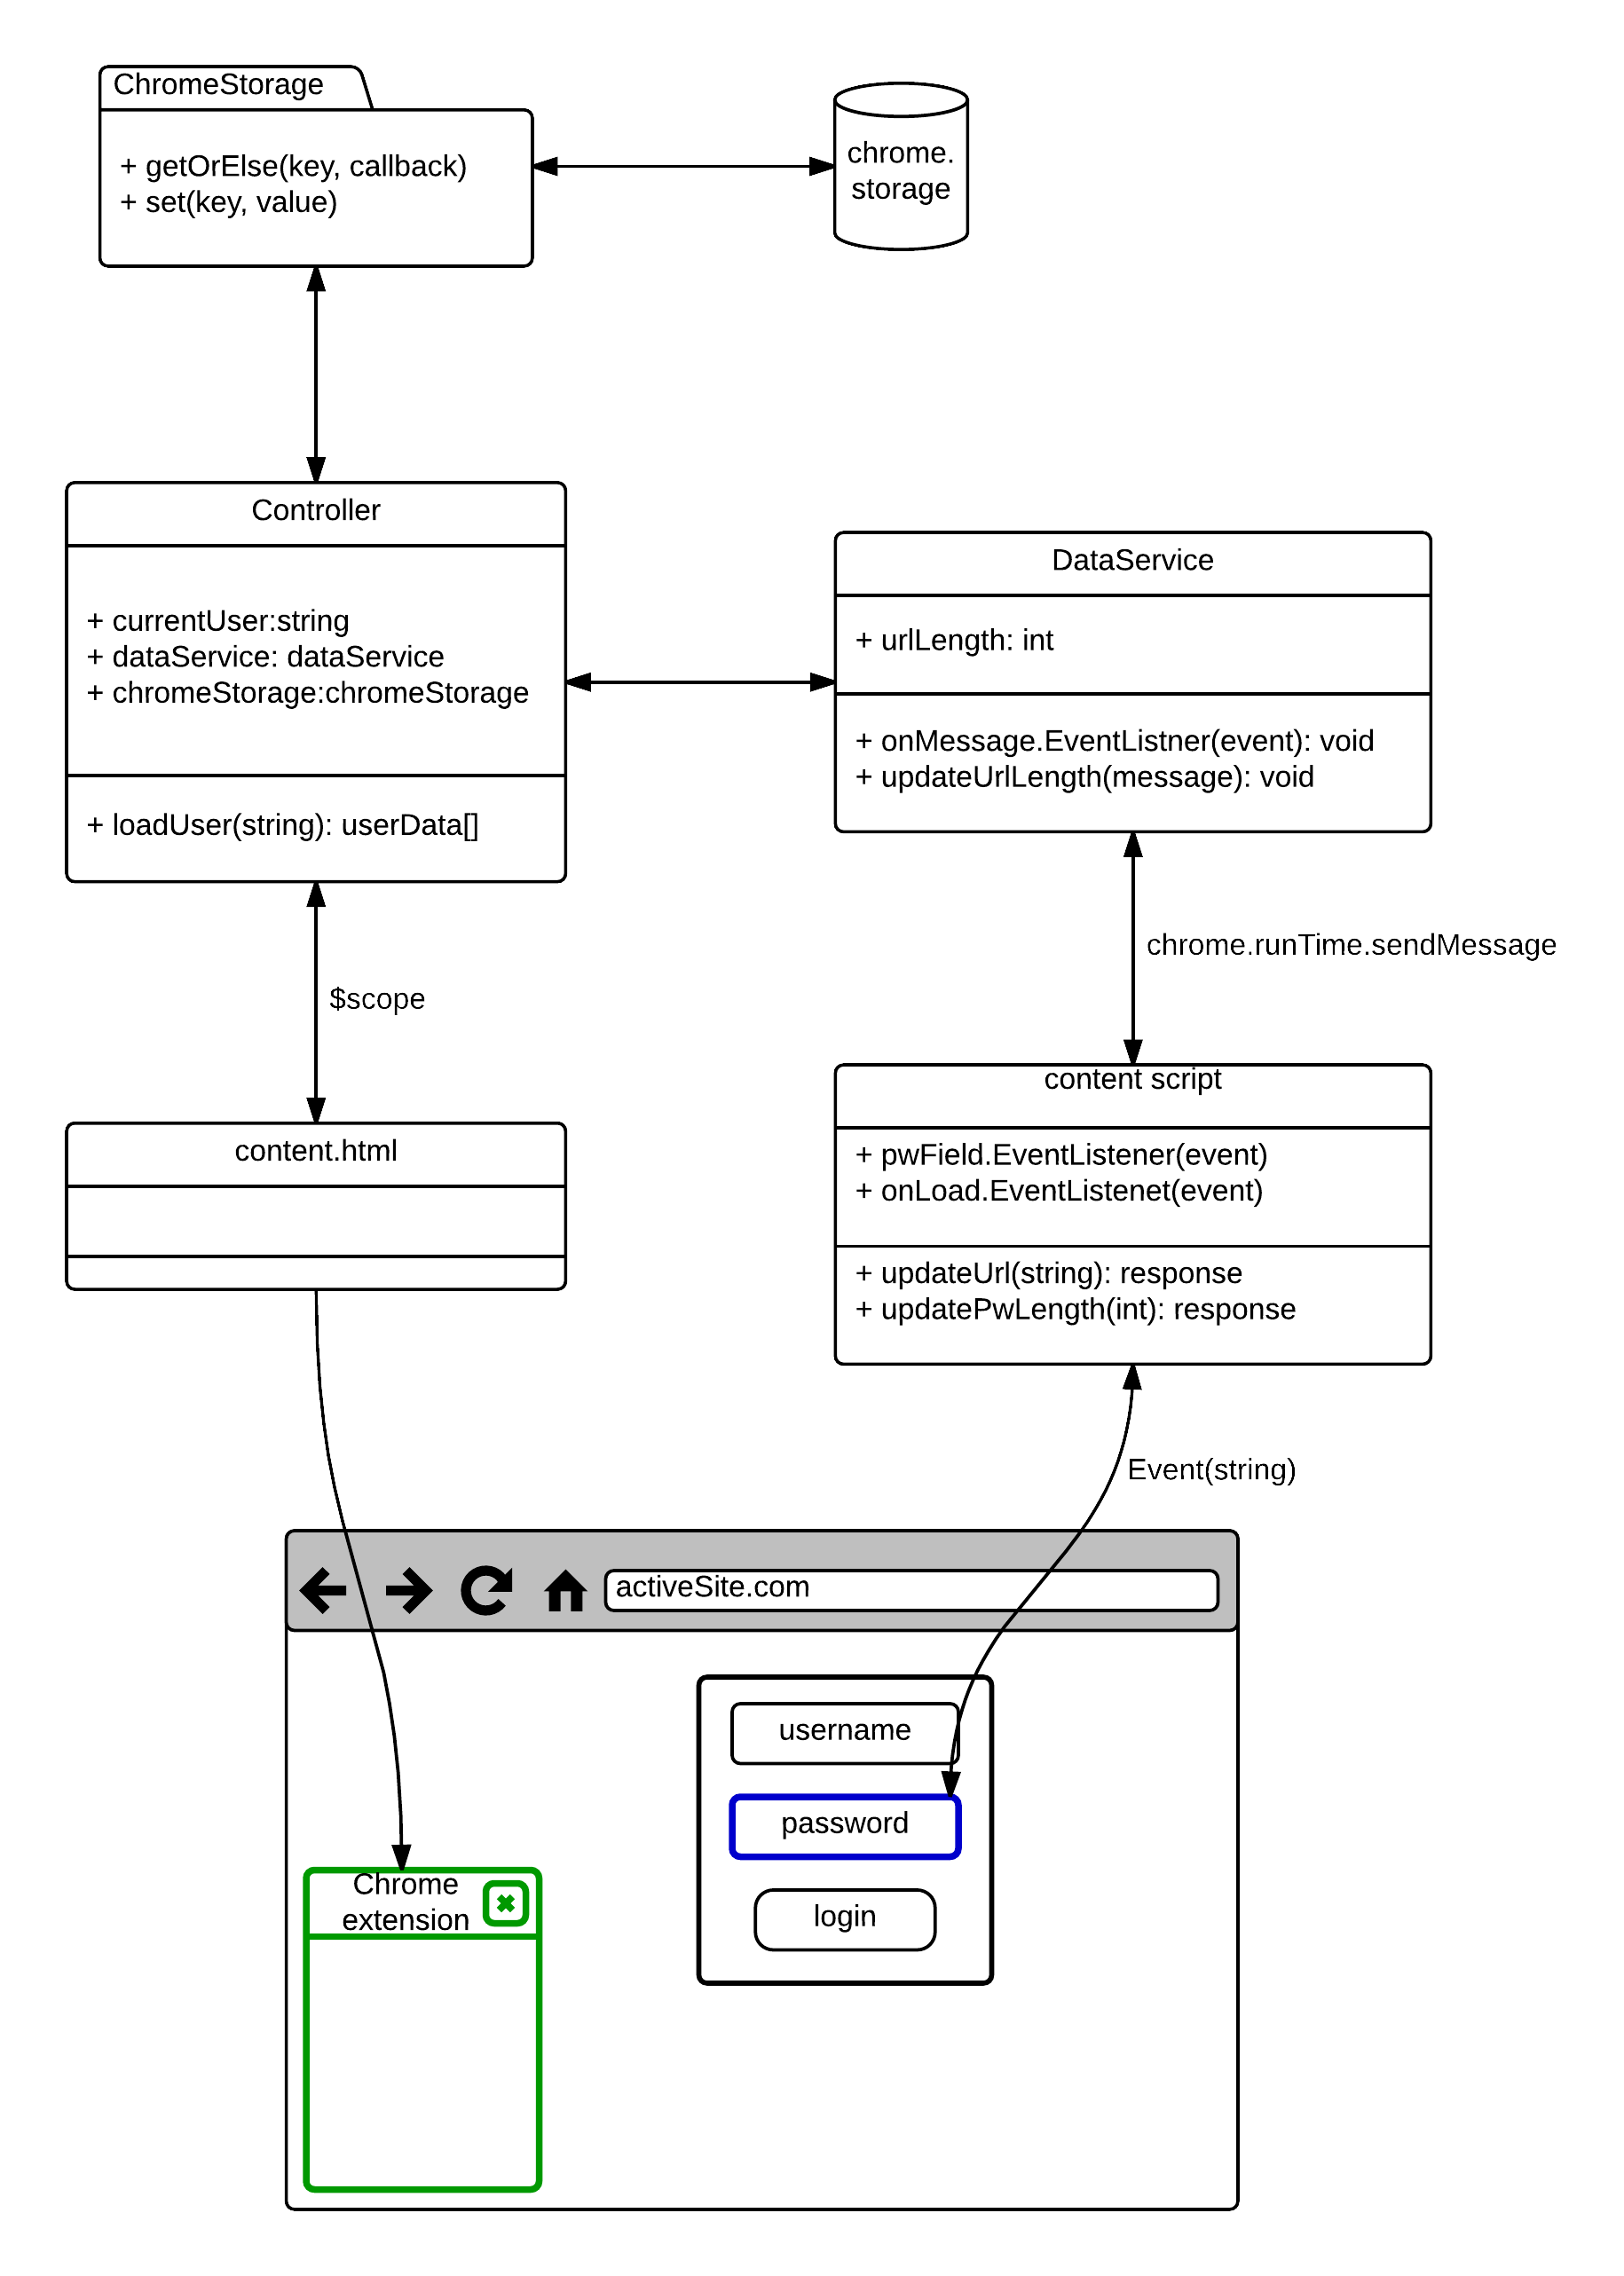
\includegraphics[width=\textwidth]{class-diagram} }
    \caption{Class diagram of the human computable passwords chrome extension.}
    \label{class-diagram}
\end{figure}
\subsection{Discussion}
\todo[inline]{Discuss how and why using an extension instead of a typical web or mobile application is more usable etc. }






